\section{Implementation Results}
\label{sec:ir}

For the implementation, it was agreed that we would create 2 separate verilog modules for the project: a display module and a timer module.

The display module is a module designed to receive a certain value and display it in the 4 7-segment displays the used FPGA offers. It has a refresh rate in order to be able to display it, as well as in order to pass by all 4 displays in order to give a simultaneous output in all 4 displays, when in reality, only one is turned on at each moment in time. This module also transforms each number in a output that draws the correct number in the 7-segment display peripheral.

The timer module is designed to count the time up to 24 hours. It has a counter variable to transform the time an instruction takes in a second, and from then on, it simply counts the seconds to make a minute and so on until it reaches the desired 24 hours and then it returns to zero. In the diagram of the Figure~\ref{fig:Timer} you can see what was explained before.

\begin{figure}[!htbp]
    \centerline{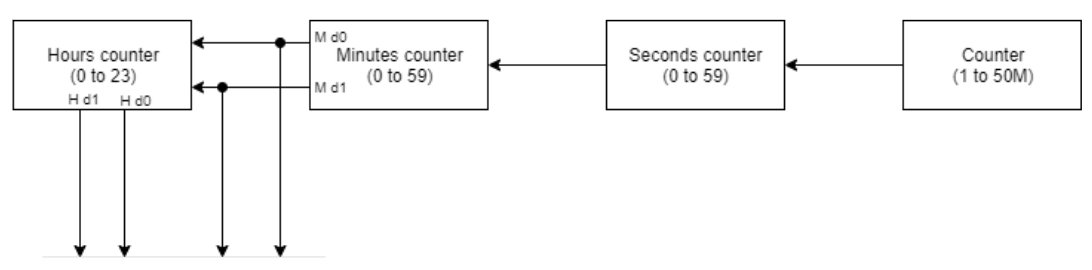
\includegraphics[width=15cm]{figures/83318261_480857235875450_5951662157752958976_n.png}}
    \vspace{0cm}\caption{Timer Diagram}
    \label{fig:Timer}
\end{figure}


For this project, we concluded that it was not necessary to create a separate module for the push button inputs.

In order to use all these peripherals and modules, they need to be added to the xtop and xaddr\_decoder verilog modules present in picoversat.

The programming part of the project was made using the C to assembly compiler provided by the teacher. However, the resulting code exceeded the memory available in picoversat. With this, adjustments to the memory were needed, and it was decided to doouble the available memory space in picoversat. This was done by changing the ADDR\_W number, on the xdefs.vh file, as well as the addresses dependant on this value.


At the end of the project deadline, the clock was able to sucessfully count up to 24 hours and display it in the FPGA, with a single continous dot in the middle to separate the hours from the minutes. However the push buttons were not able to be implemented. To finish, we put a picture of our timer running before completing another 24 hour cycle, Figure~\ref{fig:demo}. 

\begin{figure}[!htbp]
    \centerline{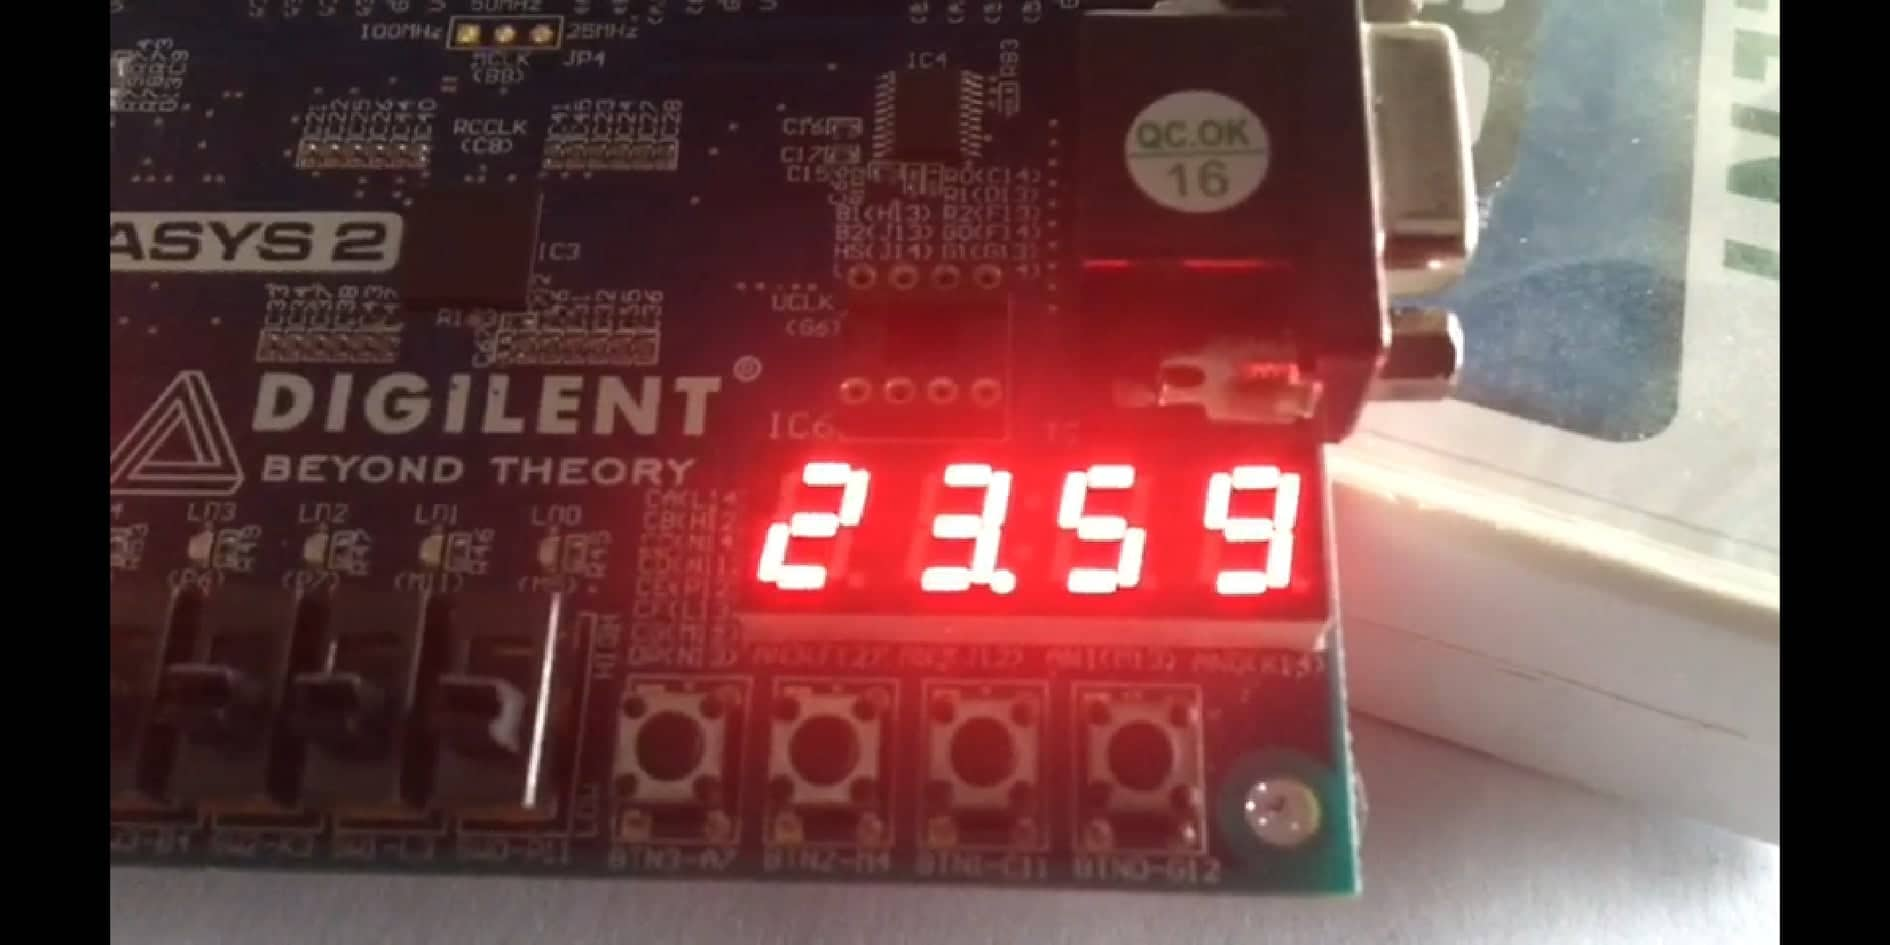
\includegraphics[width=10cm]{figures/83404584_861004010988746_2998693844775600128_n.jpg}}
    \vspace{0cm}\caption{Timer Demonstration}
    \label{fig:demo}
\end{figure}